\documentclass{hw_template}

\title{\huge\sffamily\bfseries Залікова Робота з Бази даних та інформаційних систем}
\author{\Large\sffamily Захаров Дмитро}
\date{\sffamily 28 листопада, 2024}

\begin{document}

\pagestyle{fancy}

\maketitle

\begin{center}
    \textbf{Варіант 5}
\end{center}

\tableofcontents

\pagebreak

\section{Завдання 1: Мережева Модель}

\begin{problem}
    Мережна модель даних. Відмінність простої і складної мережних структур. Переваги
та недоліки мережних структур
\end{problem}

\textbf{Відповідь.} Мережева модель даних була дуже поширеною на певному етапі
розвитку баз даних і досі використовується в деяких системах. Вона подібна до
ієрархічної моделі, оскільки також складається з набору записів, які можуть бути
власниками або членами групи, але головна відмінність полягає в тому, що один
запис у мережевій моделі може бути частиною кількох груп одночасно. Кожна група
має свою назву, а типи групових відносин відрізняються від їхніх конкретних
екземплярів. Тип визначає спільні характеристики для всіх екземплярів, а сам
екземпляр є записом-власником із підлеглими елементами. При цьому обмеження
таке: один запис не може одночасно бути частиною двох груп одного типу.

У цій моделі будь-які елементи можуть бути пов’язані один з одним, а підлеглий
запис може мати більше одного власника. Це дозволяє підтримувати зв’язки типу
``багато-до-багатьох''. Щоб спростити мережеву структуру, можна додати надмірні
дані, що дозволяє створити дерево через дублювання деяких елементів.

Іноді така надмірність є прийнятною, але в деяких випадках вона може бути
значною. Методи, що добре працюють для деревовидних структур, часто не підходять
для мережевих моделей, через що програми для обробки дерев не можуть працювати з
мережею.

Ситуацію ускладнює те, що методи, які застосовуються до одного виду мережевої
структури, можуть бути неефективними для іншого виду. Суттєвим мінусом мережевої
моделі є необхідність суворого дотримання фізичної структури даних, що ускладнює
організацію запитів. Однак її ключова перевага -- можливість створювати складні
моделі, які краще відповідають реальним процесам. Щоб зменшити складність
ієрархічної та мережевої моделей, було розроблено реляційну модель.

\textbf{Переваги та недоліки.} Сильні сторони мережевої моделі — це її ефективність у використанні пам'яті та
швидкість обробки. У порівнянні з ієрархічною, мережева модель точніше
відображає предметну область завдяки додатковим зв’язкам між елементами. Проте
серед її мінусів — складність у використанні через жорстку схему. Контроль
цілісності даних у мережевій моделі послаблений через можливість довільних
зв’язків, і при зміні даних часто потрібно змінювати програмне забезпечення. 

\textbf{Відмінність простої і складної мережних структур.} 
\begin{table}[H]
    \centering
    \begin{tabular}{|c|c|}
        \hline
        \textbf{Проста мережева структура} & \textbf{Складна мережева структура} \\
        \hline
        Відображає зв'язки ``один-до-багатьох'' & Відображає зв'язки ``багато-до-багатьох''. \\
        Має чітку ієрархію між вузлами & Один вузол пов'язаний із декількома іншими \\
        Легша у розробці та підтримці & Вимагає більш складного управління. \\
        Менш гнучка у вираженні складних відносин & Гнучкіша для моделювання складних систем \\
        \hline
    \end{tabular}
\end{table}

\newpage

\section{Завдання 2: JOIN операції}

\begin{problem}
    \texttt{INNER JOIN} та \texttt{FULL JOIN} в \texttt{SQL}.
\end{problem}

\textbf{Відповідь.} 

\textbf{INNER JOIN.} \texttt{INNER JOIN} повертає тільки ті записи, які мають
відповідності в обох таблицях. Якщо в одному з таблиць немає відповідності для
певного запису, то цей запис виключається з результатів.

Синтаксис цієї команди наведений нижче:
\begin{lstlisting}[language=SQL]
SELECT columns
FROM table1
INNER JOIN table2
ON table1.column = table2.column;    
\end{lstlisting}

\textbf{Приклад.} Нехай в нас є дві таблиці. Перша --- це таблиця \texttt{EMPLOYEES}.

\begin{center}
    \begin{tabular}{|c|c|c|}
        \hline
        \texttt{ID} & \texttt{NAME} & \texttt{DEPARTMENT\_ID} \\
        \hline
        1 & Ivan & 101 \\
        2 & Olena & 102 \\
        3 & Pavlo & NULL \\
        4 & Svitlana & 104 \\
        \hline
    \end{tabular}
\end{center}

Друга таблиця --- \texttt{DEPARTMENTS}:

\begin{center}
    \begin{tabular}{|c|c|}
        \hline
        \texttt{ID} & \texttt{DEPARTMENT\_NAME} \\
        \hline
        101 & IT \\
        102 & HR \\
        103 & Sales \\
        \hline
    \end{tabular}
\end{center}

Тоді запит може виглядати так:
\begin{lstlisting}[language=SQL]
SELECT EMPLOYEES.NAME, DEPARTMENTS.DEPARTMENT_NAME
FROM EMPLOYEES
INNER JOIN DEPARTMENTS
ON EMPLOYEES.DEPARTMENT_ID = DEPARTMENTS.ID;
\end{lstlisting}

Результатом буде наступна таблиця:
\begin{center}
    \begin{tabular}{|c|c|}
        \hline
        \texttt{NAME} & \texttt{DEPARTMENT\_NAME} \\
        \hline
        Ivan & IT \\
        Olena & HR \\
        \hline
    \end{tabular}
\end{center}

\texttt{INNER JOIN} повернув тільки записи, які мають відповідності між
\texttt{DEPARTMENT\_ID} у таблиці \texttt{EMPLOYEES} та \texttt{ID} у таблиці
\texttt{DEPARTMENTS}. Запис із \texttt{DEPARTMENT\_ID = NULL} та запис у таблиці
\texttt{DEPARTMENTS} з \texttt{ID = 103} були виключені.

\textbf{FULL JOIN.} \texttt{FULL JOIN} повертає всі записи з обох таблиць. Якщо
запис у одній таблиці не має відповідності в іншій, відповідні колонки
заповнюються значенням \texttt{NULL}. Синтаксис виглядає наступним чином:
\begin{lstlisting}[language=SQL]
SELECT columns
FROM table1
FULL JOIN table2
ON table1.column = table2.column;
\end{lstlisting}

Як приклад для таблиць вище, нехай маємо наступний запит:
\begin{lstlisting}[language=SQL]
SELECT EMPLOYEES.NAME, DEPARTMENTS.DEPARTMENT_NAME
FROM EMPLOYEES
FULL JOIN DEPARTMENTS
ON EMPLOYEES.DEPARTMENT_ID = DEPARTMENTS.ID;
\end{lstlisting}

Результатом буде наступна таблиця:

\begin{center}
    \begin{tabular}{|c|c|}
        \hline
        \texttt{NAME} & \texttt{DEPARTMENT\_NAME} \\
        \hline
        Ivan & IT \\
        Olena & HR \\
        Pavlo & NULL \\
        Svitlana & NULL \\
        NULL & Sales \\
        \hline
    \end{tabular}
\end{center}

Таким чином, \texttt{FULL JOIN} повернув усі записи з обох таблиць: 
\begin{itemize}
    \item Записи з таблиці \texttt{EMPLOYEES}, які не мали відповідностей у
    \texttt{DEPARTMENTS} (наприклад, Pavlo та Svitlana).
    \item Записи з таблиці \texttt{DEPARTMENTS}, які не мали відповідностей у
    \texttt{EMPLOYEES} (наприклад, Sales).
\end{itemize}

Таким чином, має наступну порівняльну таблицю:

\begin{center}
    \begin{tabular}{|c|c|}
        \hline
        \texttt{INNER JOIN} & \texttt{FULL JOIN} \\
        \hline
        Повертає тільки записи з відповідністю & Повертає всі записи з обох таблиць \\
        Виключає записи без відповідностей & Заповнює \texttt{NULL} для записів без відповідностей. \\
        Результат зазвичай менше & Результат зазвичай більше \\
        \hline
    \end{tabular}
\end{center}

Також, візуалізувати процес поєднання множин можна за допомогою картинки нижче:
\begin{figure}
    \centering
    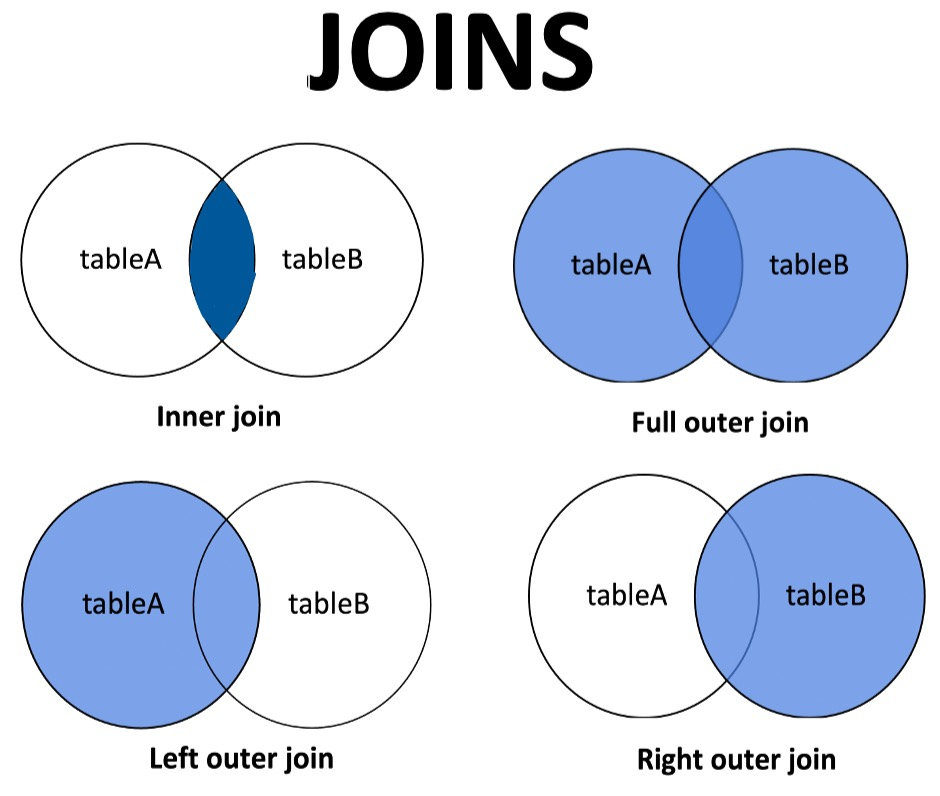
\includegraphics[width=0.7\textwidth]{joins.jpg}
    \caption{Порівняння \texttt{INNER JOIN} та \texttt{FULL JOIN}}
\end{figure}

\newpage 

\section{Завдання 3: Regex}

\begin{problem}
    Пошук рядка, що не починається з цифри
\end{problem}

\textbf{Відповідь.} Створимо дуже просту таблицю та заповнимо її даними:

\begin{lstlisting}[language=SQL]
-- Creating the test table
CREATE TABLE TEST (
    ID INT PRIMARY KEY,
    NAME VARCHAR(100)
);

-- Inserting some random data
INSERT INTO TEST (ID, NAME)
VALUES
(1, 'Ivan Kovaly'),
(2, 'Olena Sidorenko'),
(3, '123Dmytro Tkach'),
(4, 'Pavlo Shevchenko'),
(5, '3Oksana Dovgan'),
(6, 'Roman Kovtun');
\end{lstlisting}

У \texttt{SQL} можна використовувати оператор \texttt{NOT LIKE} для перевірки,
що рядок не починається з цифри. Для цього використовуємо регулярні вирази (для 
MySQL використовуємо \texttt{REGEXP}):
\begin{lstlisting}[language=SQL]
SELECT * FROM TEST
WHERE NAME NOT REGEXP '^[0-9]';
\end{lstlisting}

У \texttt{Postgres} можна використати ще більш короткий запит:
\begin{lstlisting}[language=SQL]
SELECT * FROM TEST
WHERE NAME !~ '^[0-9]';
\end{lstlisting}

Так чи інакше, задана команда обирає усі рядки, в яких поле \texttt{NAME} не
починається з цифри. Результат виглядатиме наступним чином:

\begin{center}
    \begin{tabular}{|c|c|}
        \hline
        ID & NAME \\
        \hline
        1 & Ivan Kovaly \\
        2 & Olena Sidorenko \\
        4 & Pavlo Shevchenko \\
        6 & Roman Kovtun \\
        \hline
    \end{tabular}
\end{center}

Якщо ж ми хочемо зробити regex саме під умову ``не починається з цифри'', то
регулярний вираз стає дещо складнішим: 
\begin{lstlisting}
^(?!^[0-9].*$).*
\end{lstlisting}

В такому разі, наступний запит дасть той самий результат:
\begin{lstlisting}[language=SQL]
SELECT * FROM TEST
WHERE NAME REGEXP '^(?!^[0-9].*$).*';
\end{lstlisting}

\newpage

\section{Завдання 4: Групування та середні}

\begin{problem}
    Дана таблиця \texttt{SALES} з стовбчиками: 
    \begin{itemize}
        \item \texttt{ID} --- id агента,
        \item \texttt{AGENT} --- агент (прізвище та ім’я),
        \item \texttt{ORDERNUMBER} --- номер замовлення,
        \item \texttt{ORDERDATE} --- його дата,
        \item \texttt{ORDERSUM} --- його сума.
    \end{itemize}
    Написати SQL запит, що виводить середнi суми замовлень за кожний день по
    агентам (8 балів).
\end{problem}

\textbf{Відповідь.} Спочатку, пропонується створити таблицю і накидати 
в неї деякі дані:
\begin{lstlisting}[language=SQL]
-- Creating the table itself
CREATE TABLE SALES (
    ID INT PRIMARY KEY,
    AGENT VARCHAR(100),
    ORDERNUMBER INT,
    ORDERDATE DATE,
    ORDERSUM DECIMAL(10, 2)
);

-- Inserting some data
INSERT INTO SALES (ID, AGENT, ORDERNUMBER, ORDERDATE, ORDERSUM)
VALUES
(1, 'Dimon Davis', 8805, '2023-07-18', 5000),
(2, 'Dimon Davis', 8806, '2023-07-18', 7000),
(3, 'Dimon Davis', 8807, '2023-07-19', 5000),
(4, 'Dimon Davis', 8809, '2023-07-19', 5100),
(5, 'Kate Kate', 8810, '2023-07-19', 5000),
(6, 'Kate Kate', 8816, '2023-07-19', 20000);
\end{lstlisting}

Тепер, як і просить завдання, напишемо SQL запит, що виводить середні суми
замовлень за кожний день по агентам. Для цього скористаємося командою 
\texttt{GROUP BY} разом з командою \texttt{AVG}:
\begin{lstlisting}[language=SQL]
SELECT AGENT, ORDERDATE, AVG(ORDERSUM) AS AVG_ORDER_SUM
FROM SALES
GROUP BY AGENT, ORDERDATE
ORDER BY ORDERDATE, AGENT;
\end{lstlisting}

Як результат для наданих даних отримаємо наступне:

\begin{center}
    \begin{tabular}{|c|c|c|}
        \hline
        AGENT & ORDERDATE & AVG\_ORDER\_SUM \\
        \hline
        Dimon Davis & 2023-07-18 & 6000.00 \\
        Dimon Davis & 2023-07-19 & 5050.00 \\
        Kate Kate & 2023-07-19 & 12500.00 \\
        \hline
    \end{tabular}
\end{center}

Якщо в задані просто малось на увазі вивести середню суму замовлень за кожний
день, то можна використати наступний більш простий запит:
\begin{lstlisting}[language=SQL]
SELECT ORDERDATE, AVG(ORDERSUM) AS AVG_ORDER_SUM
FROM SALES
GROUP BY ORDERDATE
ORDER BY ORDERDATE;
\end{lstlisting}

В такому разі, результат буде наступним:

\begin{center}
    \begin{tabular}{|c|c|}
        \hline
        ORDERDATE & AVG\_ORDER\_SUM \\
        \hline
        2023-07-18 & 6000.00 \\
        2023-07-19 & 8775.00 \\
        \hline
    \end{tabular}
\end{center}

\end{document}